\documentclass[../../../main.tex]{subfiles}

\begin{document}

\section{Homothety}

\begin{theorem}{Monge's Theorem}{Monge's Theorem}
The pairwise external similitude centers of three distinct circles
are collinear.
\end{theorem}
\begin{proof}
First, consider the following diagram.
\begin{figure}[H]
\centering
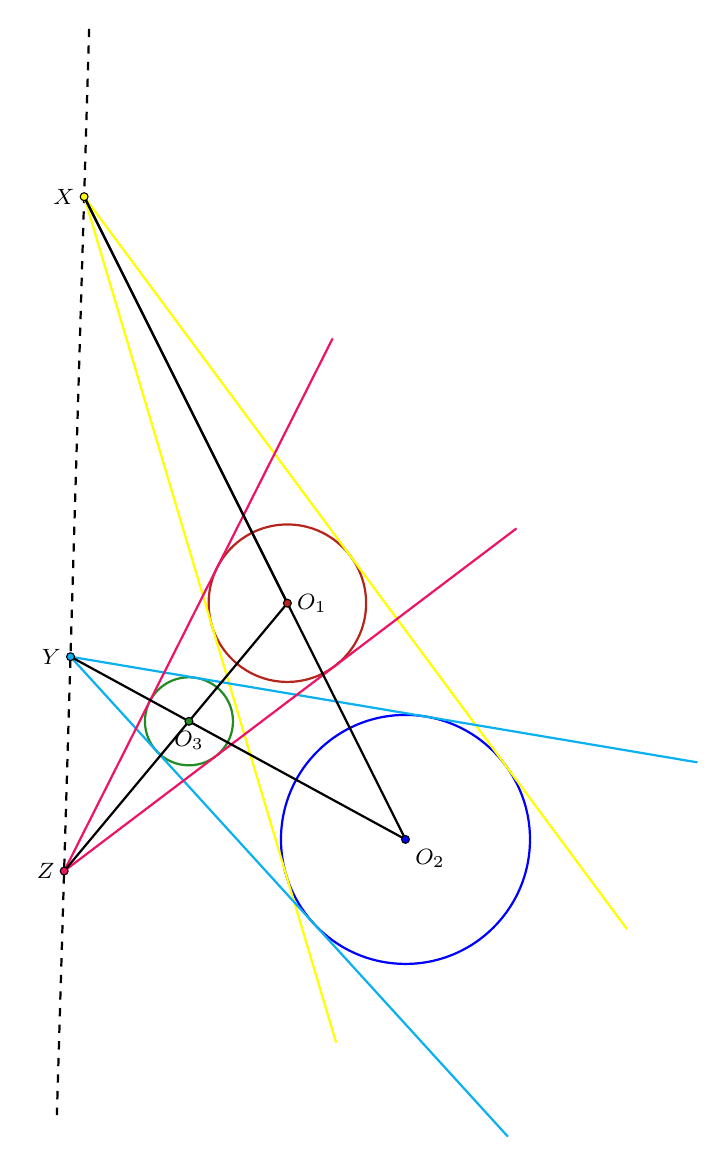
\begin{tikzpicture}[scale=0.25]
    \coordinate (O1) at (2,6);
    \coordinate (O2) at (8,-6);
    \coordinate (O3) at (-3,0);
    \coordinate (X) at (-8.324555320336787,26.649110640673555);
    \coordinate (Y) at (-9.016099767458295,3.28150896406816);
    \coordinate (Z) at (-9.338305413636002,-7.6059664963632);
    \coordinate (p1) at (4.478594673677544,-16.332420408971092);
    \coordinate (p2) at (19.249018279089587,-10.556561633949324);
    \coordinate (p3) at (13.203687791113277,-21.098898672680008);
    \coordinate (p4) at (22.831624730646023,-2.085863926492911);
    \coordinate (p5) at (4.30151507882518,19.451649497871916);
    \coordinate (p6) at (13.641555474983383,9.799845807662326);
    \coordinate (p7) at (-8.07,35.18);
    \coordinate (p8) at (-9.71,-20.01);

    \draw[thick,BrickRed] (O1) circle (4);
    \draw[thick,Blue] (O2) circle (6.324555320336759);
    \draw[thick,ForestGreen] (O3) circle (2.23606797749979);
    \draw[thick,dashed] (p7) -- (p8);
    \draw[thick,Yellow] (X) -- (p1);
    \draw[thick,Yellow] (X) -- (p2);
    \draw[thick,ProcessBlue] (Y) -- (p3);
    \draw[thick,ProcessBlue] (Y) -- (p4);
    \draw[thick,WildStrawberry] (Z) -- (p5);
    \draw[thick,WildStrawberry] (Z) -- (p6);
    \draw[thick] (O1) -- (X);
    \draw[thick] (O1) -- (Z);
    \draw[thick] (O2) -- (X);
    \draw[thick] (O2) -- (Y);

    \draw[fill=BrickRed] (O1) circle (0.2)
        node[right] {\footnotesize $O_1$};
    \draw[fill=Blue] (O2) circle (0.2)
        node[below right] {\footnotesize $O_2$};
    \draw[fill=ForestGreen] (O3) circle (0.2)
        node[below] {\footnotesize $O_3$};
    \draw[fill=Yellow] (X) circle (0.2)
        node[left] {\footnotesize $X$};
    \draw[fill=ProcessBlue] (Y) circle (0.2)
        node[left] {\footnotesize $Y$};
    \draw[fill=WildStrawberry] (Z) circle (0.2)
        node[left] {\footnotesize $Z$};
\end{tikzpicture}
\end{figure}

From the diagram above, it is evident that $X,Y,Z$ are collinear
if and only if Menelaus' Theorem holds for $\triangle{O_1O_2O_3}$.
In other words, it suffices to show that the following equation holds.
\[
\frac{O_2 X}{O_1 X} \cdot \frac{O_3 Y}{O_2 Y} \cdot
    \frac{O_1 Z}{O_3 Z}
= 1
\]
Note that $\frac{O_2 X}{O_1 X} = \frac{R_2}{R_1}$ by similar triangle.
Similarly, $\frac{O_3 Y}{O_2 Y} = \frac{R_3}{R_2}$ and
$\frac{O_1 Z}{O_3 Z} = \frac{R_1}{R_3}$. Because $\frac{R_2}{R_1}
\cdot \frac{R_3}{R_2} \cdot \frac{R_1}{R_3} = 1$, the theorem holds.
\end{proof}


\end{document}

O1 O2 O3 01
  X  Y  Z

